\section{Methods}

A set of HRV nonlinear indices were obtained, namely, Sample Entropy (SampEn), and $\alpha1$ and $\alpha2$ from the Detrended Fluctuation Analysis (DFA).  These indices were obtained for 5 minutes during resting conditions before exercising (stage 1), for the last phase of the `All Out' step (stage 2), for the first 2 minutes of the recovery step (stage 3), for the first 3 minutes of the recovery step (stage 4) and for the 5 minutes of the recovery step (stage 5). Furthermore, for the rest time, besides the cumulative measurements, the indices were obtained by using a sliding window of 3 minutes length with 1 minute overlapping, therefore obtaining two consecutive sets of indices (stage 4' and stage 5' respectively).

\subsection{Normalized Compression Distance}
here your code

\subsection{Sample Entropy}
Entropy-based methods provide a quantification of the irregularity of a temporal series. Among them, SampEn~\cite{richman00}, which is a modification of the Approximate Entropy~\cite{pincus91}, holds some properties which are appropriate for the study of physiological signals. The SampEn is the negative natural logarithm of the conditional probability that two sequences which are similar for $m$ points remain similar for $m+1$ points. Thus, a lower value of SampEn indicates more self-similarity in the time series. SampEn is robust to noise and outliers, and accordingly, it has been widely applied for characterizing the HRV signal~\cite{richman00}.

The DFA is a well-established method for assessing and quantifying fractal correlation properties in time series with non-stationarities~\cite{peng95}. This algorithm determines the scaling behavior of a time series based on the computation of a scaling exponent, $\alpha$. HRV signals have been found to show, at least, bi-scaling (bi-fractal) behavior. Therefore, two scaling exponents are needed in order to characterize the fractal correlations properties of  HRV signals, one for short-term (between 3 and 16 beats), denoted by $\alpha1$, and the other for long-term (between 16 and 64 beats), denoted by $\alpha2$.
To obtain $\alpha2$ we took into consideration that $N/4$, where $N$ is the signal length, had to be greater than the highest scale, this is, 64~\cite{Kantelhardt02}. The shortest signal length considered was 2 minutes, given that the HR populational mean  in that interval was 157 bpm, it yielded 314 beats in 2 minutes. Note that in these conditions, this requirement was tightly fulfilled for the shortest segments, and results for this index have to be examined with caution. We checked visually that the double slope and the disruption point were adequately quantified, and that low bias model in the linear regression adjustment was present. 

\begin{figure*}[!t]
\centering
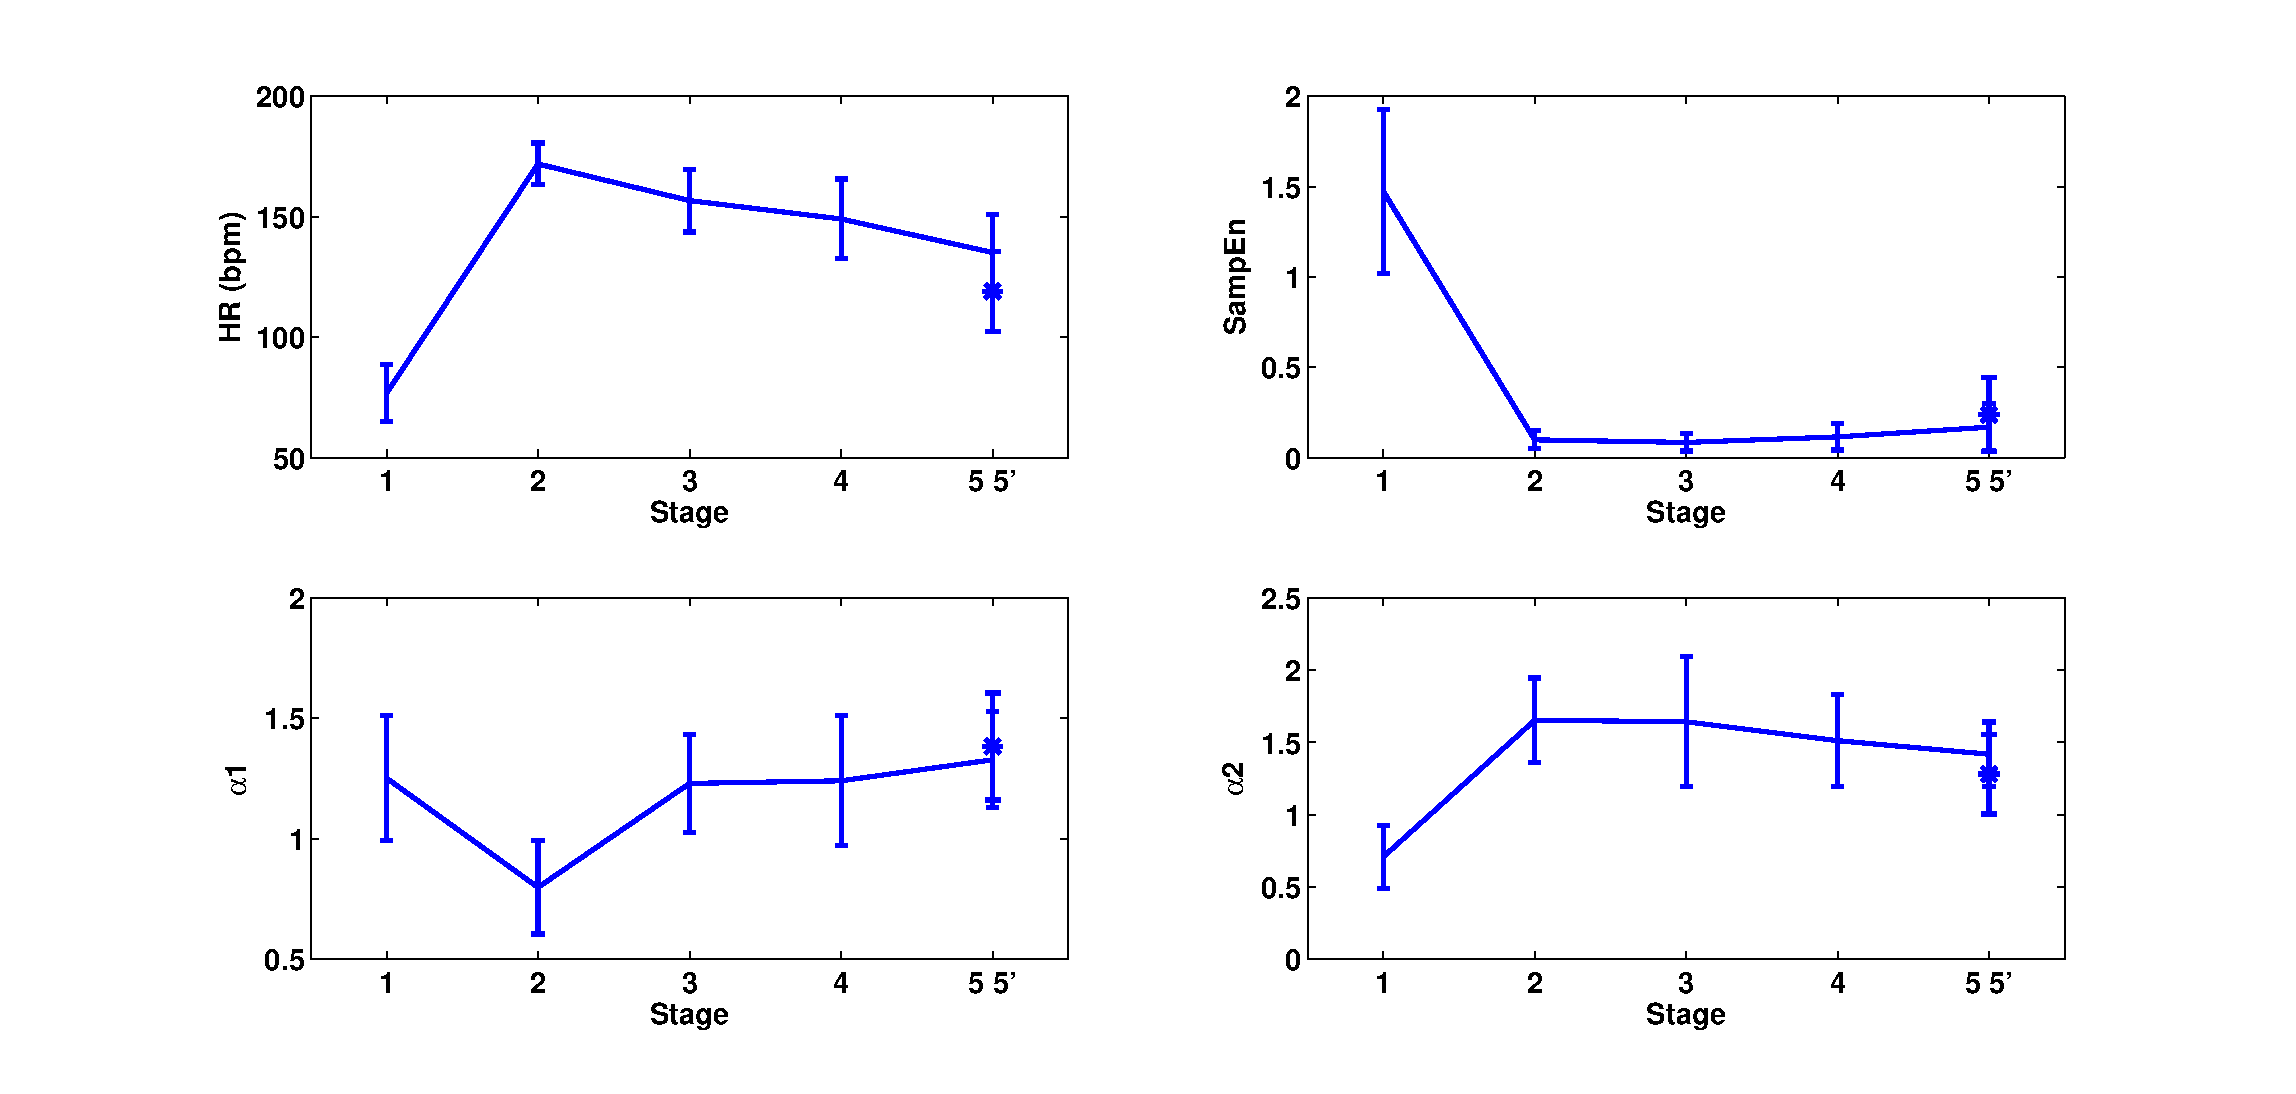
\includegraphics[width=16cm]{./figs/indicesvsHR.eps}
\caption{Mean HR (top left) and HRV indices: SampEn (top right), $\alpha1$ (bottom left), $\alpha2$ (bottom right), mean $\pm$ standard deviation, for each stage.}
\label{fig:indicesvsHR}
\end{figure*}

\begin{figure*}[!t]
\centering
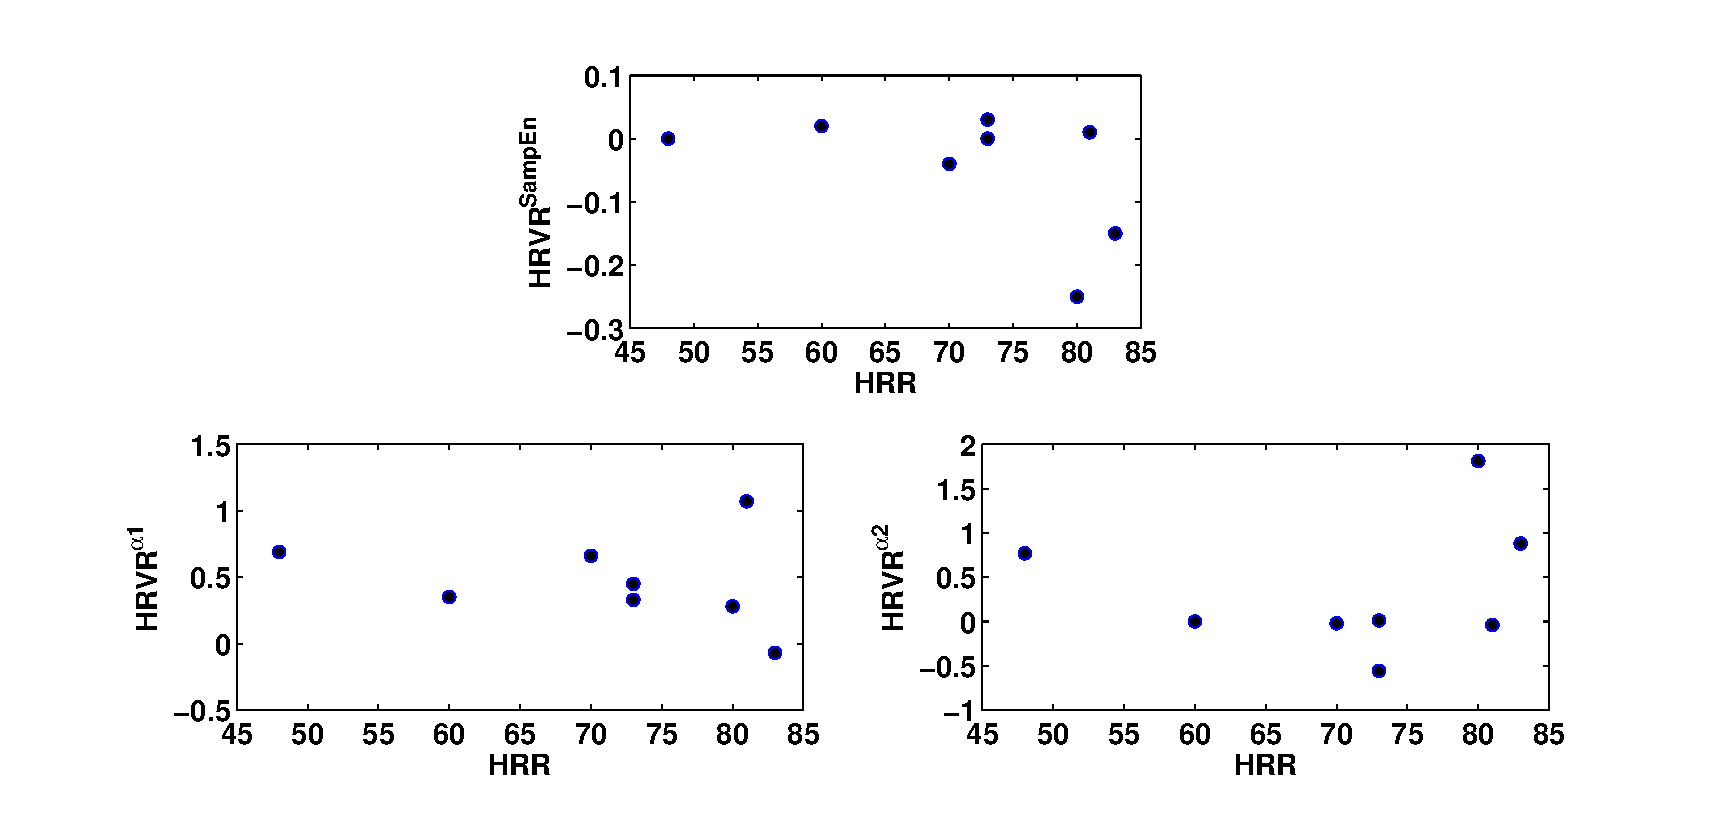
\includegraphics[width=16cm]{./figs/HRRvsHRVR.eps}
\caption{HRR vs HRVR for stage 5: SampEn (top), $\alpha1$ (bottom left), $\alpha2$ (bottom right).}
\label{fig:HRRvsHRVR}
\end{figure*} 


Mean HR of each stage was obtained for comparison.
We also obtained the HRR, which is commonly used as a marker of physical condition and even of cardiovascular risk. HRR was defined as
\[HRR = HR_{max} - HR_{min}\]
where $HR_{max}$ stands for the HR average from the last 5 seconds from the `All Out' stage, and $HR_{min}$ stands for the HR average from the last 5 seconds of the recovery time.


\begin{figure}[t]
\centering
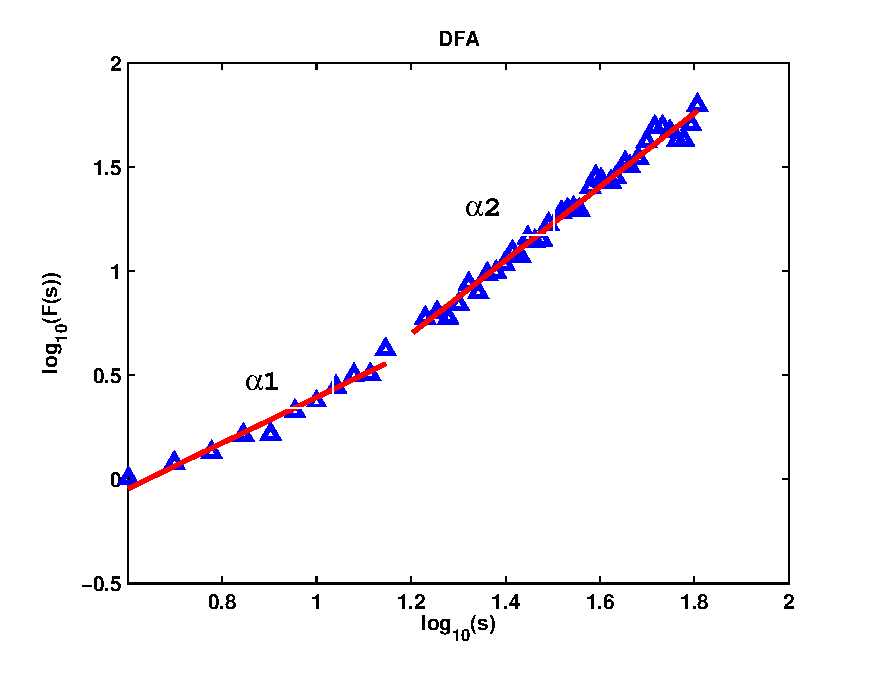
\includegraphics[width=0.4\textwidth]{./figs/alphas.eps}
\caption{Example of $\alpha1$ and $\alpha2$ computation for one of the 2 minutes segment.}
\label{fig:alphas}
\end{figure} 


Furthermore, in order to quantify HRVR and to compare it with HRR, we calculated a new  HRVR measurement, which can be obtained for any HRV index $I$, and can be defined as
\[HRVR^I = \left\{ \begin{array}{rl}
 HRV^I_{EN}- HRV^I_{RN} &\mbox{ if $HRV^I_{EN} \leq 1$} \\ 
 HRV^I_{RN}- HRV^I_{EN} &\mbox{if $HRV^I_{EN} > 1$}
       \end{array} \right.\]
where
\[HRV^I_{EN} = \frac{HRV^I_E}{HRV^I_B};  HRV^I_{RN} = \frac{HRV^I_R}{HRV^I_B}\]
and where $HRV^I_B$ stands for the basal value of the HRV index $I$; $HRV^I_E$ stands for the HRV index value of the `All Out' stage; and $HRV^I_R$ stands for the HRV index value of the recovery time. A particular HRV index $I$ may increase or may decrease with exercising, depending on what it measures, therefore, the taxonomy into two cases according to $HRV^I_{EN}$ value is made in order to achieve always a measurement indicating increasing HRV recovery when its value increases.  This makes comparison and benchmarking straightforward.
